\section{Coordination Approaches}
\subsection{Overview}
To be executable, each DSML defines a behavioral semantics. The specification of the behavior semantics of a DSML varies from natural language to the use of a formal language. In any case, the developing of complex applications relies on heterogeneous DSMLs thus resulting in heterogeneous behavioral models. In this context, Model coordination is a modeling approach to integrate the behavior of models. It proposes to specify the interaction between heterogeneous behavioral models by relying on a \emph{model of coordination}. According to \cite{coordsignibib}, ``\textit{Coordination is the process of building programs by gluing together active pieces}''. In this thesis, we adopt the wording of \emph{coordination} as being the explicit modeling of the interactions amongst behavioral models to obtain the emerging system behavior. In this sense, the coordination must be executable to enable the evaluation of the emerging behavior of the whole system. 
Coordination approaches have two major characteristics:
\begin{itemize}
	\item The interactions between models is defined separately from the computation of each model. 
	\item The individual behavior of models is kept while the coordination only constraints theirs behaviors. 
\end{itemize}
In this section, we present an overview of approaches that coordinate the behavior of models and languages. We categorize them into \emph{Coordination Languages and Architecture Description Languages} and \emph{Coordination Frameworks}. The former enables a system designer to model the coordination between models whereas the latter provides a tool to automate the coordination between models. In frameworks, the coordination is specified between heterogeneous languages.

Coordination Languages have been proposed by Carriero et al.~\cite{coordsignibib} in order to model the coordination between heterogeneous behavioral models. Depending the entities coordinated, approaches can be categorized into \emph{data-driven} or \emph{control-driven}. The former coordinates data between models whereas the latter coordinates events between models. Arbab~\cite{whatdocoord} propose to classify the approaches into \emph{endogenous} and \emph{exogenenous} languages. An endogenous language provides coordination primitives that must be incorporated within a model for its coordination. For instance, Linda~\cite{lindabib} provides a set of primitives like \emph{in()} or \emph{out()} to exchange data between models. This primitives must be added to a host language by using libraries. Conversely, in exogenous coordination languages, the coordination is isolated from the models. General speaking, these approaches rely on the notion of interface that enables to homogenize the behavior of models. The coordination is specified between elements of the interface. Manyfold~\cite{manifoldbib} and Esper~\cite{esperbib} are control-driven and exogenous languages. More precisely, they rely on an interface made of events and the coordination is specified as constraint between events. The main benefice of control driven exogenous languages is that enable a system designer to coordinate behavioral models without changing the current implementation.

In parallel, the \emph{software architecture} research field dealt with the growing complexity of software system by proposing languages (named ADL for Architecture Description Languages) to gain abstraction, structuring and reasoning capabilities~\cite{rapidebib,wrightbib,uniconbib,frameadlsbib,garlansoftarchbib}. An ADL usually specifies a system in terms of \emph{components} and interactions among those components. They enable a system designer to:
\begin{itemize}
	\item Clarify structural and semantics difference between components and interactions, 2) to reuse and compose architectural elements.
	\item Reuse and compose architectural elements.
	\item Identify/enforce commonly used patterns (\eg architectural styles).
\end{itemize}
Depending on the ADL, a \emph{Component} can for instance be an encapsulation of some procedure, an encapsulation of an object file or a (formal) abstraction of its behavior. To externally characterize the components, ADLs rely on well identified \emph{Component Interfaces}. The interfaces are used by \emph{Connectors} whose behavior is specified by a \emph{glue}. Connectors can represent a large variety of interactions (\eg procedure call, event broadcast or database queries) and the glue can range from a simple function to complex protocols. 

Both coordination languages and ADLs make a clear separation between two design activities: the specification of the component (\ie the computational aspects) and the assembly of these components (\ie the communication/coordination aspects). While the first activity is usually done by a software engineer, the second one is done by a system designer. He has to deal with the architecture-level communication that is expressed with complex protocols. To abstract away these protocols and make them reusable, ADLs propose connectors as types~\cite{frameadlsbib} that can be used on the shelf to specify domain specific interactions.

For example, Clara~\cite{clarabib} is an ADL dedicated to real time systems. It proposes built-in connector types like \emph{Rendez-vous}, \emph{Mutex} or \emph{Mailboxes}. This helps the task of a system designer by providing relevant domain specific connectors. However, this also limits what can appear in the interaction. 

\begin{figure}
\begin{center}
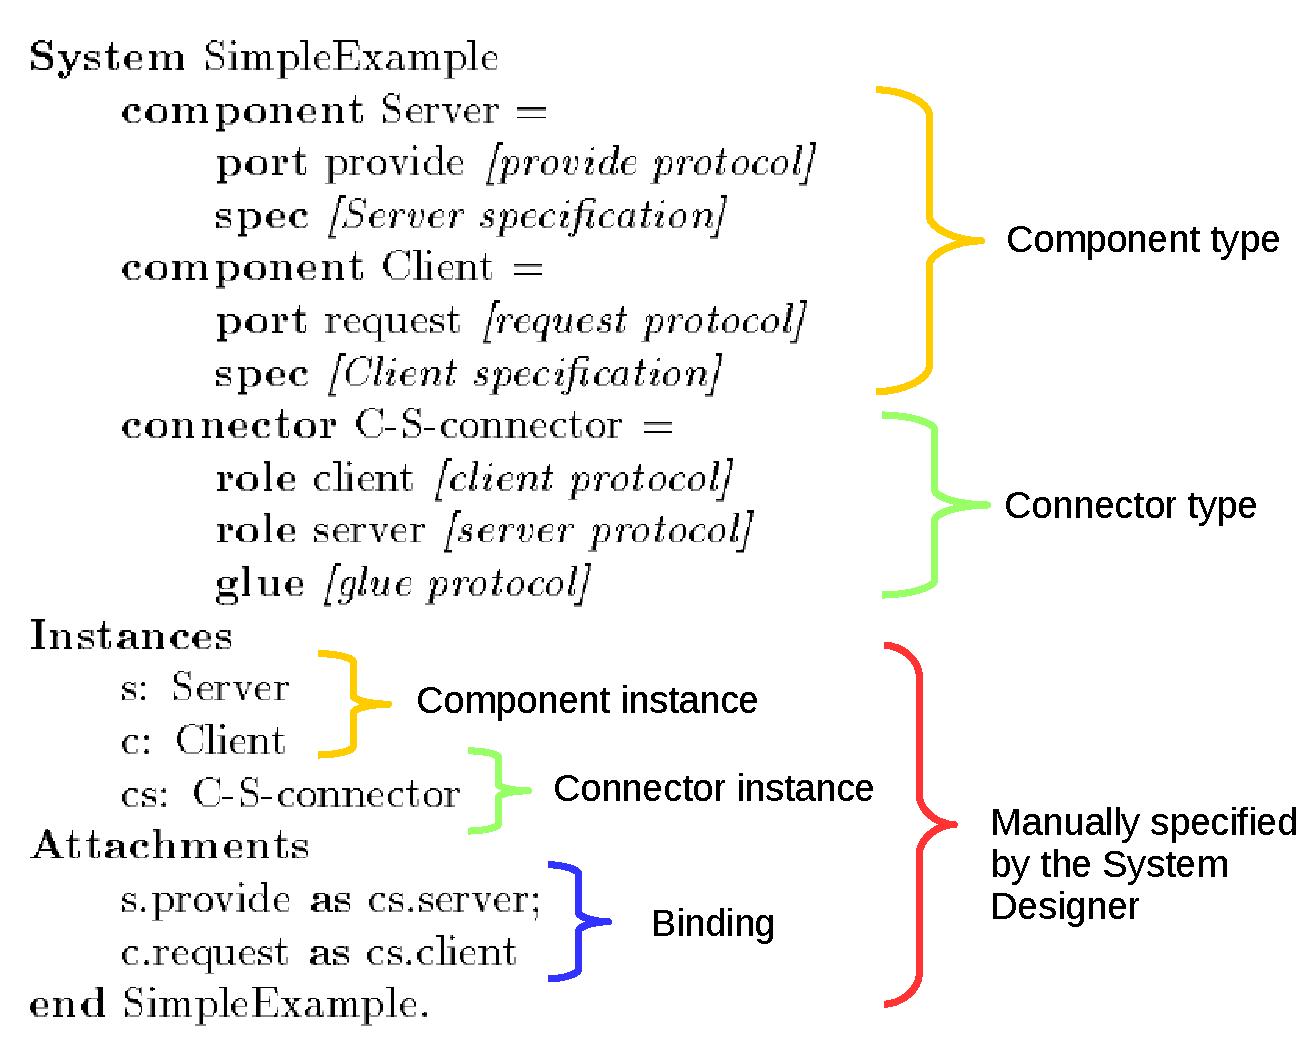
\includegraphics[width=0.5\textwidth]{background/figs/wrightspec}
\caption{Specification of a Client-Server system in Wright~\cite{wrightbib}}
\label{fig:wrightspec}
\end{center}
\end{figure}

Other approaches introduced the notion of \emph{user defined type}~\cite{uniconbib,wrightbib,reobib} that enables a system designer to build connectors for an specific domain. A connector type is defined by a set of \emph{roles} and a \emph{glue specification}. Roughly speaking, a role represents a formal parameter that is used to specify the glue. The glue is based on a formal language to specify how roles are coordinated. For instance, in Wright~\cite{wrightbib}, the glue is specified in a variant of CSP~\cite{csphoarebib}, whereas in Reo it is specified by the composition of dedicated primitives~\cite{reobib}. The connector types are later on instantiated and the roles are bound to the actual interfaces of the instances of components. 

To illustrate how a system designer can define a set of domain specific connector types, Figure~\ref{fig:wrightspec} shows a simple client-server system described in Wright~\cite{wrightbib}. The specification defines two component types named \emph{Client} and \emph{Server}, and one connector type named \emph{C-S-connector}. The C-S-connector has two roles (\emph{client} and \emph{server}) and a glue that describes how the activities of the client and server roles are coordinated. The section \emph{Instances} describes a particular configuration by instantiating the corresponding components and connectors. The example describes a system where there is a single server (\emph{s}), a single client (\emph{c}) and a single connector (\emph{cs}). Then, the section \emph{Attachments} defines which component ports are attached to the connector roles. 

The major drawback of Coordination Languages and ADLs is that they coordinate is specified between models. For instance, in the case of ADLs, a system designer has to instantiate and bind connector types manually. Returning to the example of Figure~\ref{fig:wrightspec}, for each server and client in the system, the system designer has to instantiate two components and one connector. Then, he has to bind the component ports with the connector roles. With the increasing number and heterogeneity of the components, this task can quickly becomes difficult and error prone.

\emph{Coordination Frameworks} identified that the instantiation and binding of connector types can be a systematic activity the system designer repeats many times and can consequently be defined as a pattern. Such a pattern is based on the know-how of the system designer and sometimes on naming or organizational conventions adopted by the models. Thus, they have captured the specification of a behavioral coordination pattern inside a tool/framework to automate the instantiation and binding of connector types. They specify the coordination between heterogeneous languages rather than between particular models (see Figure~\ref{fig:coordapp}). Such specification is then applied on models to instantiate a set of connector types and bind their instances. In this thesis, we refer to these approaches as “Coordination Pattern Approaches”.

%This example illustrates how a system designer can define a set of domain specific connector types, and then, instantiate and bind the connector types as needed by its architecture.
 


%Regarding the classification for coordination languages, ADLs are control-driven and exogenous approaches.